%%%%%%%%%%%%%%%%%%%%%%%%%%%%%%%%%%%%%%%%%%%%%%%%%%%%%%%%%%%%%%%%%%%%%%%%%%%%%%%%
%2345678901234567890123456789012345678901234567890123456789012345678901234567890
%        1         2         3         4         5         6         7         8
\documentclass[letterpaper, 10 pt, conference]{ieeeconf}  % Comment this line out if you need a4paper
\IEEEoverridecommandlockouts                              % This command is only needed if 
                                                         % you want to use the \thanks command
\usepackage[utf8]{inputenc}
\usepackage{amsmath}
\usepackage{bm}
\usepackage{amssymb}
\usepackage{graphicx}
\usepackage{booktabs}
\usepackage{mathrsfs}
\usepackage{amsbsy}
\usepackage{caption}
\usepackage{float}
\usepackage{subcaption}
\usepackage{varwidth}
\usepackage{algorithm}
\usepackage{tabularx}
\usepackage{yhmath}
\usepackage{multirow}
\usepackage{multicol}
\usepackage{booktabs}
\usepackage{rotating}
\usepackage[table]{xcolor}
\definecolor{grey}{rgb}{0.9,0.9,0.9}
\usepackage[noend]{algpseudocode}
\usepackage[top=60pt,left=48pt,right=48pt,bottom=45pt]{geometry}	
\usepackage{dsfont}
\usepackage{environ}
\usepackage[framemethod=TikZ]{mdframed}
\usepackage{algorithm}
\usepackage{accents}\newcommand\addtag{\refstepcounter{equation}\tag{\theequation}}
\usepackage{etoolbox}
\usepackage{graphicx}
\usepackage{rotating}
\usepackage{enumerate}
\usepackage[colorlinks]{hyperref}
\usepackage{relsize}
\usepackage{gensymb}
\usepackage{cleveref}
\usepackage{threeparttable}
\usepackage{xspace} 
\usepackage{colortbl}
\usepackage{siunitx}
\definecolor{Gray}{gray}{0.9}
\newcommand{\comFB}[1]{\noindent\colorbox{yellow}{\parbox{\dimexpr\columnwidth-1\fboxsep}{[FB: #1]}}}
%%% Customized commands
%%% math commands
\newcommand{\mvec}[1]{\bm{#1}}
\newcommand{\dmvec}[1]{\dot{\mvec{{#1}}}}
\newcommand{\ddmvec}[1]{\ddot{\mvec{{#1}}}}

\newcommand{\xt}{\mvec{x}(t)}
\newcommand{\ut}{\mvec{u}(t)}

% \newcommand{\st}{\text{s.t.}}  % This conflicts with soul and does not seem to be used anyway
\newcommand{\g}{\mvec{g}}
\newcommand{\q}{\mvec{q}}
\newcommand{\dq}{\dmvec{q}}
\newcommand{\ddq}{\ddmvec{q}} 

%%% table commands
\newcommand{\mymultirow}[2]{\parbox[t]{2mm}{\multirow{#1}{*}{\rotatebox[origin=c]{90}{#2}}}}
%%% Document
\title{\LARGE \bf Bioptim, a Python interface for Musculoskeletal Optimal Control in Biomechanics}
\author{Benjamin Michaud\textsuperscript{a,*,$\dagger$}, François Bailly\textsuperscript{a,$\dagger$}, Amedeo Ceglia\textsuperscript{a}, Eve Charbonneau\textsuperscript{a}, Léa Sanchez\textsuperscript{a}  and  Mickael Begon\textsuperscript{a}% <-this % stops a space

\thanks{\textsuperscript{$\dagger$}\,These authors have contributed equally to this work and share first authorship.}
\thanks{\textsuperscript{a}\,Laboratoire de Simulation et Modélisation du Mouvement, Faculté de Médecine, Université de Montréal, Laval, QC, Canada}%
\thanks{\textsuperscript{*}\,BENJAM@umontreal.ca}
}

%%% User commands

\usepackage{pdfrender}
\DeclareRobustCommand*{\pmbb}[1]{%
  \textpdfrender{
    TextRenderingMode=Stroke,
    LineWidth=.1pt,
  }{#1}%
}
\NewEnviron{comeq}{%
\par\vspace{0ex}
\begin{mdframed}[outerlinewidth=0.5,leftmargin=10,rightmargin=-10pt,backgroundcolor=white,hidealllines=true,leftline=true,
innertopmargin=0pt,splittopskip=0, skipbelow=\baselineskip, innerbottommargin=0pt%
skipabove=0ex]%
\vspace{-0ex}\hspace{0pt}\textit{Proof:}%
\itshape
\begin{equation*} 
\begin{split}
\BODY
\end{split}
\end{equation*}
\end{mdframed}
}
\newcommand{\pd}[2]{\frac{\partial #1}{\partial #2}}
\def\abs{\operatorname{abs}}
\def\argmax{\operatornamewithlimits{arg\,max}}
\def\argmin{\operatornamewithlimits{arg\,min}}
\def\diag{\operatorname{Diag}}
\newcommand{\eqRef}[1]{(\ref{#1})}
\newcommand{\dbtilde}[1]{\accentset{\approx}{#1}}
\newcommand{\state}{\mathbf{x}}
\newcommand{\dstate}{\dot{\mathbf{x}}}
\newcommand{\control}{\mathbf{u}}
\newcommand{\param}{\mathbf{p}}
\newcommand{\bioptim}{\textit{Bioptim}\xspace}
\newcommand{\casadi}{\textit{CasADi}\xspace}
\newcommand{\biorbd}{\textit{Biorbd}\xspace}
\newcommand{\acados}{\textit{ACADOS}\xspace}
\newcommand{\ipopt}{\textit{Ipopt}\xspace}
\newcommand{\bioviz}{\textit{Bioviz}\xspace}
\newcommand{\moco}{\textit{OpenSim Moco}\xspace}
\newcommand{\opensim}{\textit{OpenSim}\xspace}
\newcommand{\acado}{\textit{Acado}\xspace}
\newcommand{\gpopsii}{\textit{Gpops-II}\xspace}
\newcommand{\muscodii}{\textit{Muscod-II}\xspace}
\newcommand{\anybody}{\textit{Anybody}\xspace}
% bioptim's nomenclature
\newcommand{\constraints}{\texttt{Constraints}\xspace}
\newcommand{\constraint}{\texttt{Constraint}\xspace}
%
\newcommand{\objectives}{\texttt{Objective functions}\xspace}
\newcommand{\objective}{\texttt{Objective function}\xspace}
%
\newcommand{\dynamics}{\texttt{Dynamics}\xspace}
%
\newcommand{\bounds}{\texttt{Bounds}\xspace}
\newcommand{\bound}{\texttt{Bound}\xspace}

% Revision tools 
\usepackage{soul}  
\newcommand\comment[2]{\hl{#1}}
\newcommand\addref{\comment{REF}{}}
\newcommand\xx{\comment{XX}{}}
\hyphenpenalty=10000

\begin{document}

\maketitle
\thispagestyle{plain}
\pagestyle{plain}

\begin{abstract}
Musculoskeletal simulations are useful in biomechanics to investigate the causes of movement disorder, to estimate non-measurable physiological quantities or to study the optimality of human movement.
We introduce \bioptim, an easy-to-use Python framework for biomechanical optimal control, handling musculoskeletal models. 
Relying on algorithmic differentiation and the multiple shooting formulation, \bioptim interfaces nonlinear solvers to quickly provide dynamically consistent optimal solutions.
The software is both computationally efficient (C++ core) and easily customizable, thanks to its Python interface.
It allows to quickly define a variety of biomechanical problems such as motion tracking/prediction, muscle-driven simulations, parameters optimization, multiphase problems, etc.
It is also intended for real-time applications such as moving horizon estimation and model predictive control.
Six contrasting examples are presented, comprising various models, dynamics, objective functions and constraints. 
They include data-driven simulations (i.e., a multiphase muscle driven gait cycle and an upper-limb real-time moving horizon estimation of muscle forces) and predictive simulations (i.e., a muscle-driven pointing task, a twisting somersault with a quaternion-based model, a position controller using external forces, and a multiphase torque-driven maximum-height jump motion).
\end{abstract}

\textbf{Keywords -- Biomechanics, Optimization, Optimal control, Musculoskeletal simulation, Software}



\section{Introduction}\label{sec:introduction}
Biomechanics researchers rely on numerical simulations of motion to gain understanding on a variety of scientific topics such as the physiological causes of movement disorders and their consequences on health [\addref], the estimation of non-measurable physiological quantities (e.g., muscle forces)[\addref] and the optimality of human movement [\addref].
The musculoskeletal models used in these simulations generally have a large number of degrees of freedom and they are governed by several ordinary differential equations (ODEs) which mainly describe multibody and muscle activation dynamics.
The complexity of these systems has led scientists to formulate their simulations as optimal control problems (OCP), relying on efficient non-linear optimization software to find trajectories that fulfill a desired task while enforcing the system dynamics and minimizing a cost (e.g. motion duration, energy expenditure, matching experimental data, etc.).
Up to very recently, there was no off-the-shelf software available to the community to quickly formulate and solve such musculoskeletal OCPs. 
Consequently, researchers had to develop their own solutions, with little or no dissemination to the community, limiting  synergies between researchers.


As a result, many approaches coexist to formulate and solve OCPs in the biomechanical literature. 
The formulation, also called discretization, consists in turning a continuous trajectory optimization problem into a generic discrete non-linear program (NLP) that is solved using a dedicated algorithm. 
The main family of so-called \textit{direct} transcription methods comes from numerical optimal control. 
They consist in straightforwardly choosing the state and/or the control as optimization variables at a given number of points along the trajectory and they rely on the integration of the system dynamics between these points. 

For instance, the \textit{direct collocation} method has shown its efficiency in some studies investigating human motion [\addref\comment{, \`a prendre dans papier MOCO}{Sinon j'en ai un paquet dans mon Zotero que j'avais fait pour ma préparation de synthèse}]. 
It consists in approximating the integration of the system dynamics using polynomials that describe the state and control trajectories.
Its main advantages are that it leads to very sparse NLPs, that knowledge about the state trajectory can be used in the initialization, and that it handles unstable systems well \cite{diehl2006fast}. 
Its major disadvantage is that adaptive integration error control implies regridding the whole problem and thus changes the NLP dimensions, discarding its use for such application [\addref].
\textit{Direct multiple shooting} is another direct method that was also applied with success in a lot of biomechanics [\addref] and robotics [\addref] studies.
Its advantages are mostly the same as for direct collocation in addition to combine integration error control with fixed NLP dimensions, as it relies on possibly adaptive ODE solvers to integrate the system dynamics.
Besides direct methods, other choices can be made, as in \cite{yeadon2000mechanics} [+ \addref\ Begon], where the optimization variables are instants at which a switch in the motor strategy occurs, using polynomials function (4th, 5th order) in-between, or in \cite{leboeuf2006energetic} [+ \addref\  Huchez, Mombaur, McPhee, Opensim]], where the optimization variables are the coefficients of fourth order polynomial approximations of the states, with linking conditions to enforce the continuity of the controls. 
These last approaches are less generic than the direct methods as they either require a prior knowledge about the state and control trajectories. 
Most of the time, when investigating complex biomechanics issues, we do not have this information. 


\begin{figure}[t!]
\centering
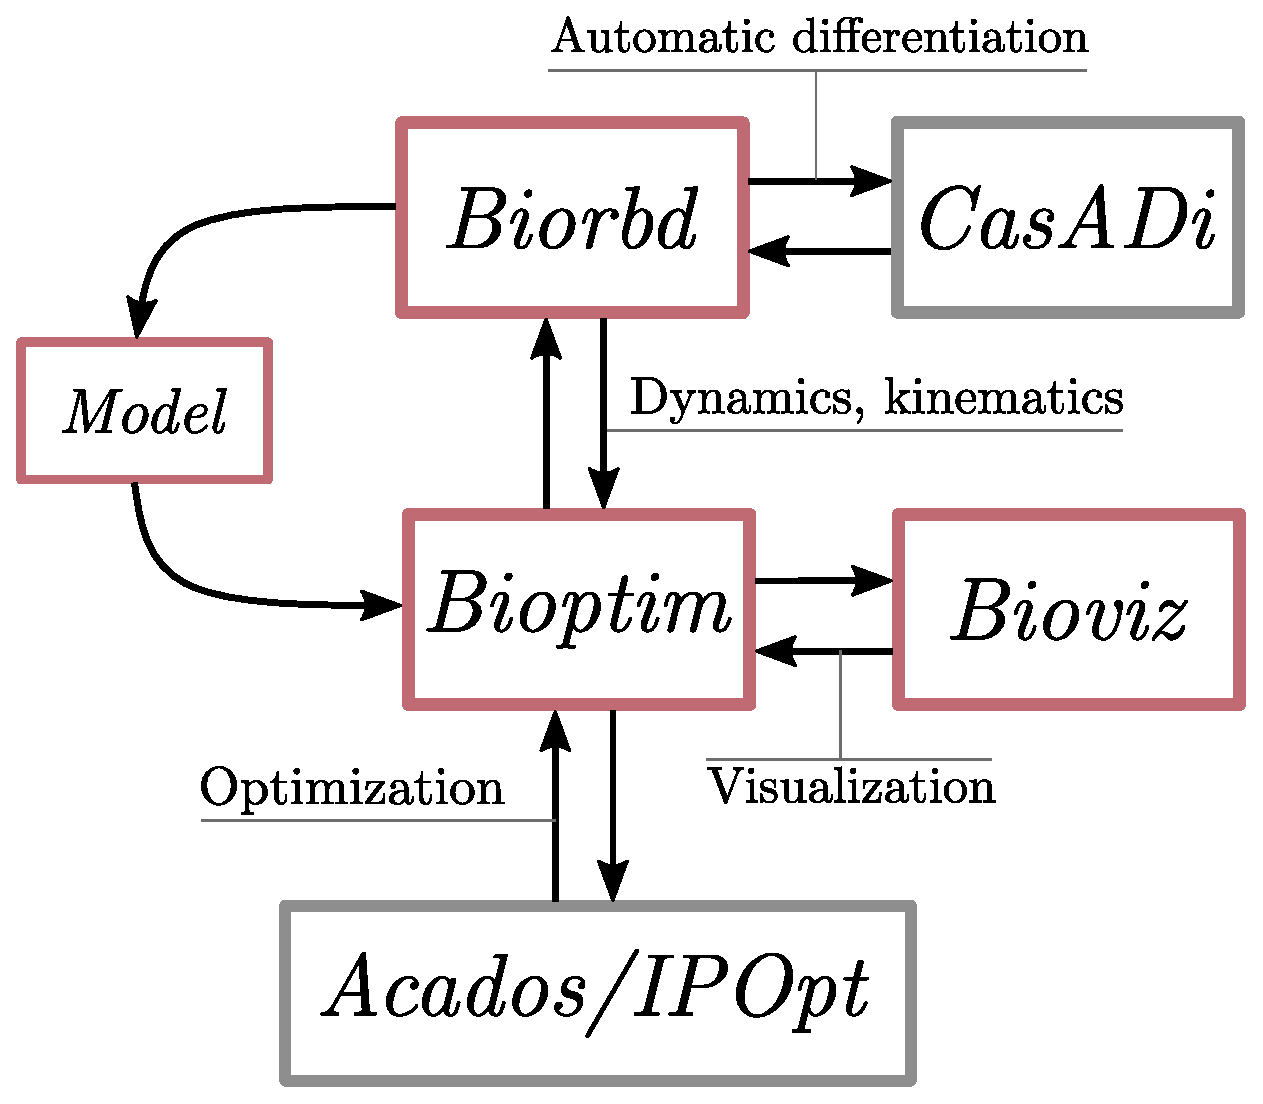
\includegraphics[width=0.9\columnwidth]{figures/dependencies.eps}
\caption{\bioptim dependencies flowchart. The red-boxed software are developed by the S2M team. The \bioptim part is further detailed in Fig.~\ref{fig:dependencies}.}
\label{fig:dependencies}
\vspace*{-0.5cm}
\end{figure}

Concerning the non-linear solver, a variety of software exist and have been used to solve transcribed musculoskeletal NLPs.
They can use different heuristics: interior point methods (\ipopt, [\addref]) or sequential quadratic programming (\textit{snopt} [\addref], \acados [\addref]), but they are all gradient based.
Therefore, derivatives of the NLP cost function and constraints are required to perform optimization.
These derivatives can be obtained by finite differences (often implemented but inaccurate thus comprising convergence) or computed exactly using automatic differentiation (requiring to write all dependencies of the software in symbolic variables) [CasADi].


In order to promote the use of musculoskeletal optimal control among biomechanics researcher, we identified a strong need for a dedicated tool, as shown by the recently launched \moco [\addref, Opensim]. 
The biomechanics community being mainly composed of software users [\addref], such a tool should request a flexible user interface written in a widely used high-level and if possible open-source language (e.g. Python) with a low-level core (e.g. C++) for efficiency. 

To develop such a software, four interrelated components are essential to us: \textit{i)} a musculoskeletal modeling software, with a visualization module (multibody kinematics and dynamics, muscle dynamics, etc.), \textit{ii)} a method for automatic differentiation, \textit{iii)} a discretization approach, and \textit{iv)} one or several nonlinear programming (NLP) solvers. 
General-purpose optimal control software (e.g. \gpopsii [\addref], \muscodii [\addref], \acado [\addref]) address \textit{ii)} to \textit{iv)} but they need to be interfaced with a musculoskeletal modeling module and they do not provide any built-in biomechanics features (physiological cost functions, kinematic constraints, etc.). 
In that sense, the aforementioned \moco, is a welcome initiative that draws its strength from its integration with the widely used \opensim.
However, it faces the following limitations: it uses finite differences to avoid the complexity of adapting the \opensim codebase to support automatic differentiation, it uses direct collocation as transcription method, preventing the use of adaptive ODE solvers and it is not as flexible as required by the community, since it requires the user to develop new features, such as new objective functions, in C++. 

The objective of the present paper is to introduce \bioptim, an open-source optimal control software dedicated to musculoskeletal biomechanics.
\bioptim is based on C++ code for computational efficiency but the user interface is written in Python for flexibility and ease-of-use. 
The OCP transcription uses direct multiple shooting to preserve the possibility of using arbitrarily accurate ODE solvers for the integration, which is fully parallelized for more efficiency.
\textit{Bioptim's} core is fully written in \casadi symbolics to benefit from algorithmic differentiation and to exploit \casadi 's interface with several non-linear solvers (\textit{ipopt, snopt}).
Moreover, \bioptim is interfaced with the cutting-edge solver \textit{acados}, a recent NLP solver dedicated to direct multiple shooting, intended for real-time applications.
The purpose of \bioptim is to allow fast and flexible musculoskeletal OCP formulation and solving by providing a framework with a lot of typical biomechanics problem already implemented and customizable.

The paper is organized as follows: first, the design and implementation of \bioptim are described.
Next, the versatility and performances of \bioptim are shown through a variety of examples available online. 


\section{Implementation and Design}\label{sec:design&impl}
\subsection{Implementation and dependencies}
\bioptim is the top layer of a series of libraries (\biorbd: dynamics and MSK modeling; \casadi: automatic differentiation; \ipopt/\acados: optimization; \bioviz: visualization).
Within this software suite, \bioptim 's main role is to shape the problem to allow its dependencies to communicate efficiently, while providing an intuitive and flexible interface to the user (Fig.~\ref{fig:dependencies}).
Therefore, it was written in Python for its flexibility and its widespread use among researchers.
However, all intensive calculations behind the interface are performed in C/C++, keeping \bioptim both fast and easy to customize.

\begin{figure}[t!]
\centering
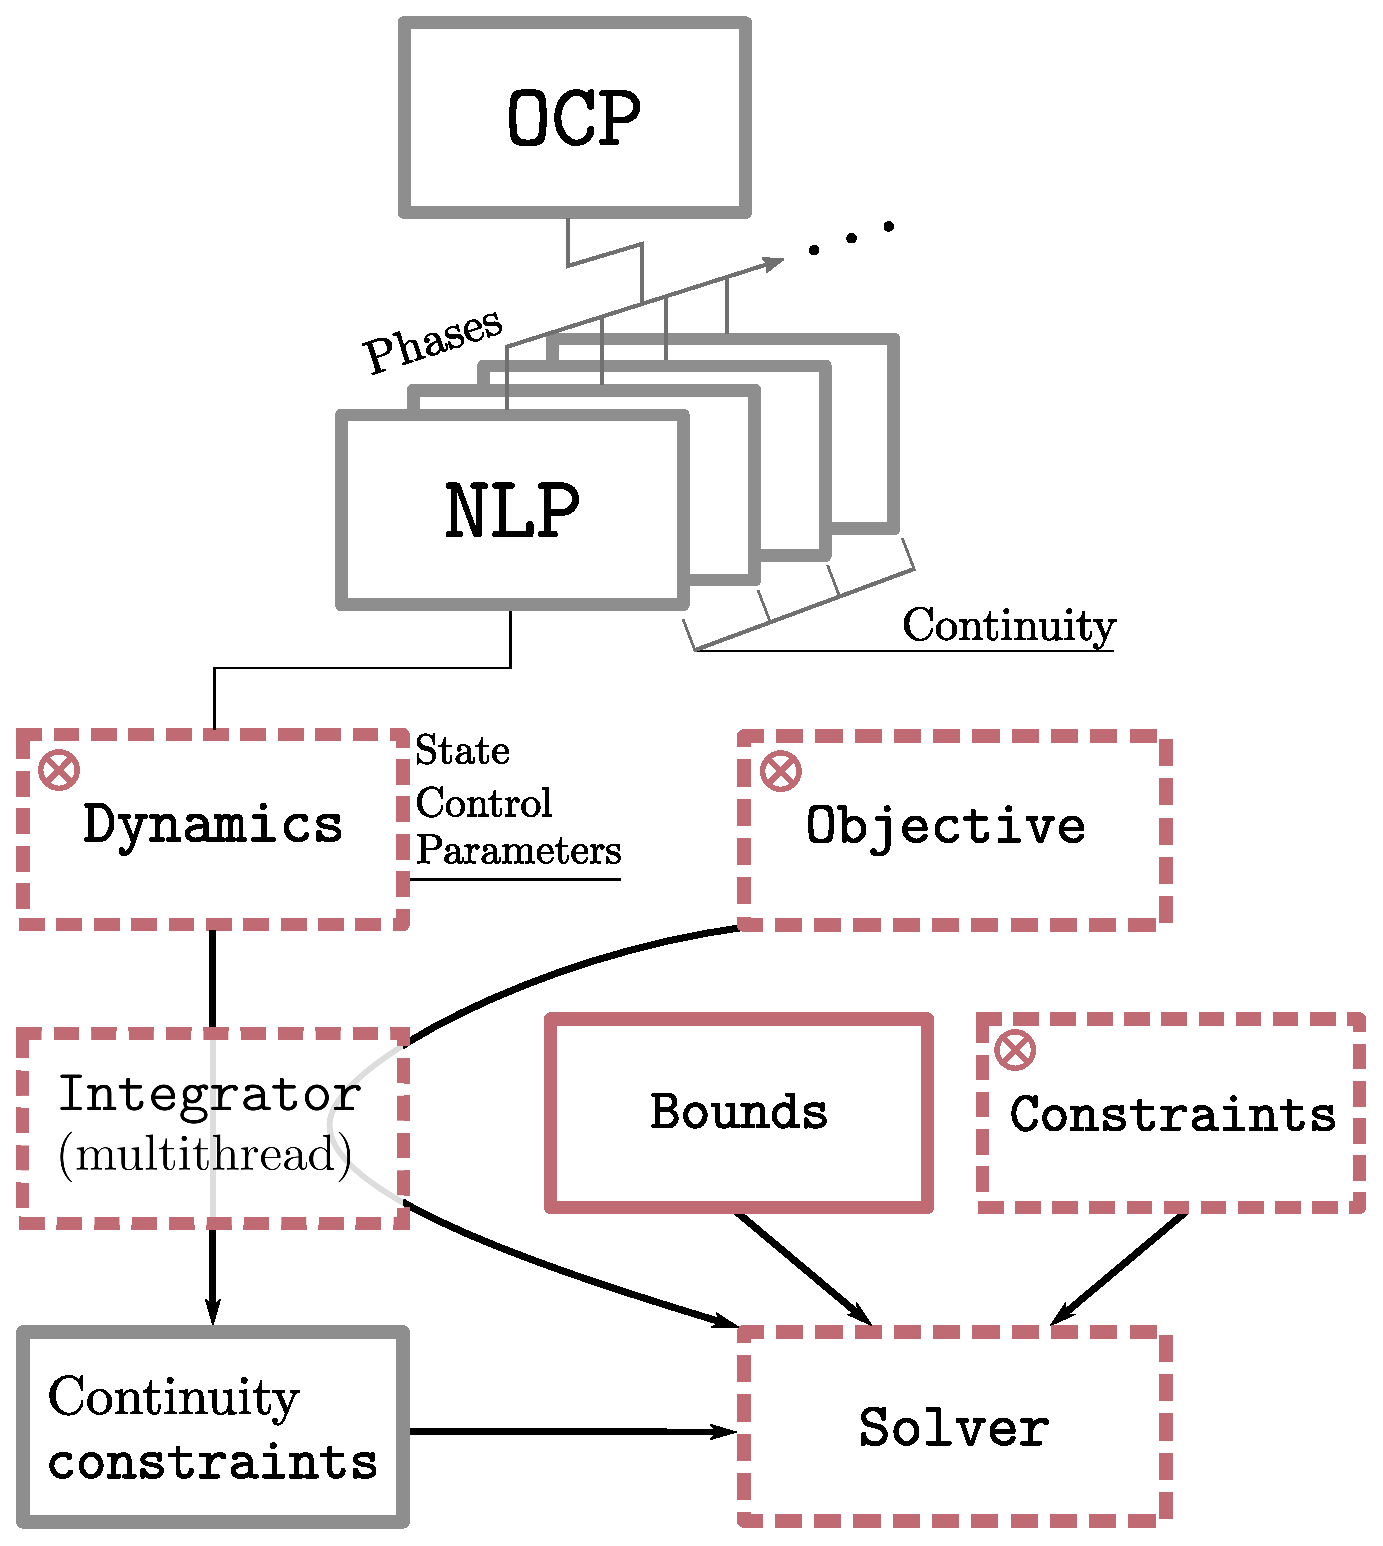
\includegraphics[width=0.9\columnwidth]{figures/design.eps}
\caption{\bioptim design flowchart. The red box correspond to objects that must be filled in by the user. The red-dashed boxes correspond to pre-implemented objects already available to the users. The * stands for easily customizable objects.}
\label{fig:flowchart}
\vspace*{-0.5cm}
\end{figure}


\subsection{Design}
\bioptim shapes and solves optimal control problems whose two required entries are a model (.\textit{bioMod} file) and an OCP.
The model file contains the geometrical characteristics and the segment inertial parameters as well as optional elements, namely, the markers, the actuators of the model (muscles and joint torques possibly with torque/angle/velocity relationships) as well as bounds on joint kinematics and torques. 
It also allows the user to design or import meshes for visualization purposes.
The \texttt{OCP} consists in a combination of nonlinear problems (NLPs) that allows for the formulation of multi-staged OCPs. 
Each \texttt{NLP} has the following attributes: \textit{1)} a dynamics type, \textit{2)} an objective function set, \textit{3)} a constraint set, \textit{4)} variables bounds, \textit{5)} a number of shooting points and the duration of the problem and \textit{6)} initial guesses.
Based on these inputs, \bioptim properly sets up the multiple shooting transcription of the OCP, with appropriate continuity constraints (between the shooting nodes and the phases) and shapes it up to feed the chosen nonlinear solver (\ipopt or \acados). 
Next, we develop the different attributes of each \texttt{NLP}:

\subsubsection{Dynamics}
The dynamics defines which variables are states ($\state$), controls ($\control$) and parameters ($\param$), the latter being time-independent.
Then, it implements the ordinary differential equation governing the state dynamics:

\[
\dstate = f(\state, \control, \param).
\addtag
\label{eq:state_transition}
\]

\noindent More than 10 dynamics are already implemented in \bioptim \footnote{\href{https://github.com/pyomeca/bioptim/blob/master/bioptim/dynamics/dynamics_functions.py}{github link}}, among which the controls can be muscle excitations, muscle activations and/or joint torques, the states can be muscle activations and/or joint kinematics.
They can include contact points, external forces, etc.
Even if these dynamics types exhaustively span the current usages in biomechanics, a custom dynamics type is also pre-implemented to easily customize problems.

\subsubsection{Objective function set}
In line with the optimal control formalism, there are two main types of objective functions, namely Lagrange and Mayer. 
Lagrange types are running objectives, integrated over the NLP duration. Mayer types are time-specific objectives. 
Classically, they correspond to a terminal objective, but to be more versatile, they can be defined at any instant in \bioptim.

Objective functions can depend on any of the optimization variable, \textit{i.e.} the controls, the states, the parameters and the duration of the problem. 
A lot of objective function types are already implemented in \bioptim ($>\!20$), among which tracking\:/\:minimizing, on states\:/\:controls\:/\:markers\:/\:contact\:forces\:/\:problem\:duration, etc. 
Should one go missing, a custom objective type is also possible to define.

When declaring the desired list of objective functions for a given NLP, each objective function type is associated with a weight, and the user can choose on which components of the vector variables the objective must apply. 
If applicable (for tracking objective functions mainly), the user must also specify the numerical target of the objective.

\subsubsection{Constraint set}
Classically, constraints are hard penalties of the optimization problem, i.e., a solution will not be considered optimal, unless all constraints (equality or inequality) are met.
The \texttt{Constraint} class contains a variety of already implemented constraints.
Some of them are specific functions, commonly useful in biomechanical problems (e.g. non-slipping contact point, non-linear bounds on torque depending on the state, etc.), the others have their equivalent in the \texttt{ObjectiveFunction} class.
Should one go missing, a custom constraint type is also possible to define.

\subsubsection{Bounds}
Essentially, the \texttt{Bounds} are constraints directly related to the states, the controls and the parameters.
They are useful for defining model-related constraints such as kinematic, torque or muscle excitation\:/\:activation limits. 

\subsubsection{Shooting points and problem duration}
In a direct multiple shooting formulation, the total duration of the problem is divided into smaller intervals whose initial values are called shooting points. 
In \bioptim, the user is asked to define a number of shooting points and a problem duration, per phase.
Possibly, the problem duration can be part of the optimization variables, allowing for, e.g., minimal time formulations.

\subsubsection{Initial guesses}
Once the problem is set up, the user can provide an \texttt{InitialGuess} for all the optimization variables, at each shooting point.
This feature aims at providing prior information to the solver.
Several \texttt{InterpolationTypes} are implemented in \bioptim (constant, linear, spline, each shooting point, etc.), to quickly let the user define the initial guesses.
A custom \texttt{InterpolationType} is also possible to implement.

\section{Examples}\label{sec:Examples}
In this section, six applications are presented to illustrate the versatility of \bioptim and give a practical overview on how to use its main features.
The settings and performances (convergence time, single shooting integration error, optimized objective) of each OCP are summarized in Tab.~\ref{tab:Perfs_and_detailed_implementations_of_each_example}. 
When possible, problems were solved with both \ipopt and \acados.
In the following, bold symbols denote vectors and starred ones ($^*$) denote reference or tracked quantities.


\subsection{Muscle activation driven pointing task}\label{ex:poiting}
%
In this first example, the goal was to achieve a muscle activation driven pointing task using a 2-DoF arm model with six muscle elements. 
In addition to muscle-induced torques, pure joint torques were added to compensate for the model weaknesses.
The main term (highest weight) of the objective function (Eq.~\ref{eq:cost_pointing}) is a Mayer objective, corresponding to the pointing tasks at the final node, to superimpose two markers, the first one ($\mathbf{m_u}$) fixed in the ulna system of coordinates and the second one ($\mathbf{m^*_s}$) fixed in the scene.
The three Lagrange terms  were added for control (muscle activation $\bf{a}$ and joint torques $\boldsymbol{\tau}$) and state ($\bf{x}$) regularization:
\[
\begin{aligned}
	\mathcal{J} = 	&~\omega_1~\underbrace{\|\mathbf{m_u}(T)-\mathbf{m^*_s}\|^2}_{\mathtt{TRACK\_MARKERS}}~\\
	&\int_{t=0}^T\underbrace{\|\bf{a}\|^2}_{\mathtt{MIN\_ACTIVATION}}~
	+\underbrace{\|\boldsymbol\tau\|^2}_{\mathtt{MIN\_TORQUE}}~
	+\underbrace{\|\bf{x}\|^2}_{\mathtt{MIN\_STATE}}~ dt,
\end{aligned}
\addtag
\label{eq:cost_pointing}
\]

\noindent where $T\!=\!\SI{2}{\second}$ is the duration of the motion, and $\omega_1\!=\!1e5$.
The problem was discretized using 50~shooting nodes with a 5-steps Runge-Kutta-4 (RK4) integration in-between.
The problem was solved using \ipopt (with exact Hessian computations) and \acados (with a Gauss-Newton approximation of the Hessian) resulting in two very close solutions.
\acados was about 50 times faster than \ipopt and was better at enforcing the continuity constraints (as shown by the single shooting error in Tab.~\ref{tab:Perfs_and_detailed_implementations_of_each_example}).
\ipopt however ended up with a smaller optimized objective (20.8 \textit{vs} 23.2), leading to a more optimal solution than \acados. 
Superimposed snapshots of the optimal motion found with \acados are displayed in Fig.~\ref{fig:snapshots_activation_driven_pointing}.
It is worth mentioning that for the purpose of this illustration, no constraint was given on the shoulder range of motion to ensure physiological muscle trajectories. 


\subsection{Quaternion base twisting somersault}\label{ex:somersault}
In this example of acrobatic sports biomechanics, the goal was to maximize the twist rotation ($\phi$) of a 8-DoF model in a backward somersault.
The model was composed of a 6-DoF root segment and two 1-DoF torque actuated shoulder joints.
Two different numerical description of the root segment rotations were used (Euler angles and quaternions).
The objective function was as follows:

\begin{eqnarray}\label{eq:ocp_Trampo}
\mathcal{J} = \omega_1 \underbrace{\int_0^T \dot{\phi}~dt}_{\mathtt{MIN\_TWIST}}  +~\omega_2 \underbrace{\int_0^T \sum_{i=1}^{2}~\tau_{i}^2~dt}_{\mathtt{MIN\_ TORQUE}},
\end{eqnarray}
with $\omega_1 = -1$ (resulting in the maximization of the first term) and $\omega_2 = 1\times 10^{-6}$, T the duration of the movement and $\tau_{i}$ the torque control input of the $i^{th}$ arm DoF.
The first term of the objective function (Eq.~\ref{eq:ocp_Trampo}) corresponds to maximizing the twist velocity and the second term serves as control regularization.


The movement lasted for approximately 1 second and was discretized with 80 shooting nodes.
The solutions for both models were \comment{similar}{ce n'est pas vraiment le cas, commenter} (Fig.~\ref{fig:snapshots_quaternion_base_twisting_somersault}) highlighting the equivalence of the two rotation representations.
Euler angles have the advantage to be easily interpretable, but they suffer from the loss of a DoF at the Gimbal lock (leading to numerical instabilities).
The use of a quaternion-based representation is tackles this numerical stability issue when a joint is free to rotate on a three-dimensional range of motion.
Quaternion's integration must be handled with care~\cite{bailly2020optimal}, which was taken care of in \textit{bioptim}.


\begin{figure*}[t!]
\centering
\includegraphics[width=\textwidth]{figures/Euler_Bioptim_MaxVrille_dos.png}\\
\vspace*{0.5em}
\includegraphics[width=\textwidth]{figures/Quat_Bioptim_MaxVrille_dos.png}
\caption{Snapshots of a maximally twisting somersault driven by shoulder torque actuators and a free base expressed by Euler angles (top) or quaternions (bottom).}
\label{fig:snapshots_quaternion_base_twisting_somersault}
\end{figure*}


% \begin{table}[h!]
% \caption{\small Objective terms of quaternion base maximally twisting somersault}
% \label{tab:Quaternion_base_twisting_somersault}
% \centering
% \begin{tabular}{c c c c}
% \toprule 
% & Type & Function & Weight \\ 
% \midrule
% $\#1$ & Lagrange & MINIMIZE\_TWIST & $-1e1$ \\ 
% \midrule
% $\#2$ & Lagrange & MINIMIZE\_ TORQUE & $1e-6$ \\ 
% \bottomrule
% \end{tabular}
% \end{table}















\subsection{Pendulum on a spring}\label{ex:spring}
\emph{\begin{figure}[t!]
\centering
\includegraphics[width=0.35\columnwidth]{figures/Mass_Pendulum_Model_2.png}
\caption{Definition of the spring-mass-pendulum model.}
\label{fig:Mass_Pendulum_Model}
\end{figure}}
This spring-mass-pendulum-based example is presented to introduce \bioptim 's ability to use external forces.
The goal was to hold the position of a $\SI{1}{\kilo\gram}$ mass hanging on a linear spring attached to the ground.
A $\SI{0.2}{\meter}$-long pendulum weighting $\SI{10}{\kilo\gram}$ was attached to the mass and free to rotate in one dimension (Fig.~\ref{fig:Mass_Pendulum_Model}).
In addition to the spring force, the mass was actuated by a vertical external force (e.g., something pulling on it) while the pendulum rotation was passive.
The system therefore comprised two DoFs, the mass position ($q_m$) and the pendulum angle ($q_p$) and one control input, the vertical external force pulling on the mass ($\tau$). 
The spring force $\mathcal{F}_s$ was:
\[
\begin{aligned}
\tau_s = -k*q_m,
\end{aligned}
\addtag
\label{eq:f_ext}
\]
with $k$ the spring stiffness constant.\\
The OCP was composed of two phases each lasting for $\SI{5}{\second}$, with 50 shooting nodes.
In the first phase, no objective function was minimized and $\tau$ was constrained to be $0$, letting the mass oscillating freely. 
Then, in the second phase, a cost function (Eq.~\ref{eq:ocp_Pendulum}) was minimized, to enforce a reference position $q_m^*$ of the mass.
This objective function, exclusively composed of Lagrange terms, was formulated as follows:
\[
\mathcal{J} = \int_{T/2}^T \underbrace{ (q_m - q_m^*)^2}_{\mathtt{TRACK\_STATE}}  +~\omega_1 \underbrace{\tau^2~dt}_{\mathtt{MIN\_ TORQUE}}~dt,
\addtag
\label{eq:ocp_Pendulum}
\]

\noindent with $q_m^* = \SI{-0.5}{\meter}$ and $\omega_1 = 10^{-6}$ and T is the duration of the movement.
The first term of the objective function (Eq.~\ref{eq:ocp_Pendulum}) acts as a position controller for the mass.
The second was added for control regularization.


During the first phase, the mass is passively oscillating around its stationary position due to the spring force (Fig.~\ref{fig:Mass_Pendulum_Fext_graphs}).
At the beginning of the second phase, when an additional external force acts on the mass, it stabilizes around the targeted position.
The standard deviation between the position and the targeted position is $\SI{0.04}{\m}$.
This example highlights the possibility of using optimal control to find activation patterns compensating for external passive forces (e.g., ortheses flexibility, contact surface deformation, interaction between two models, etc.).

\begin{figure*}[t!]
\centering
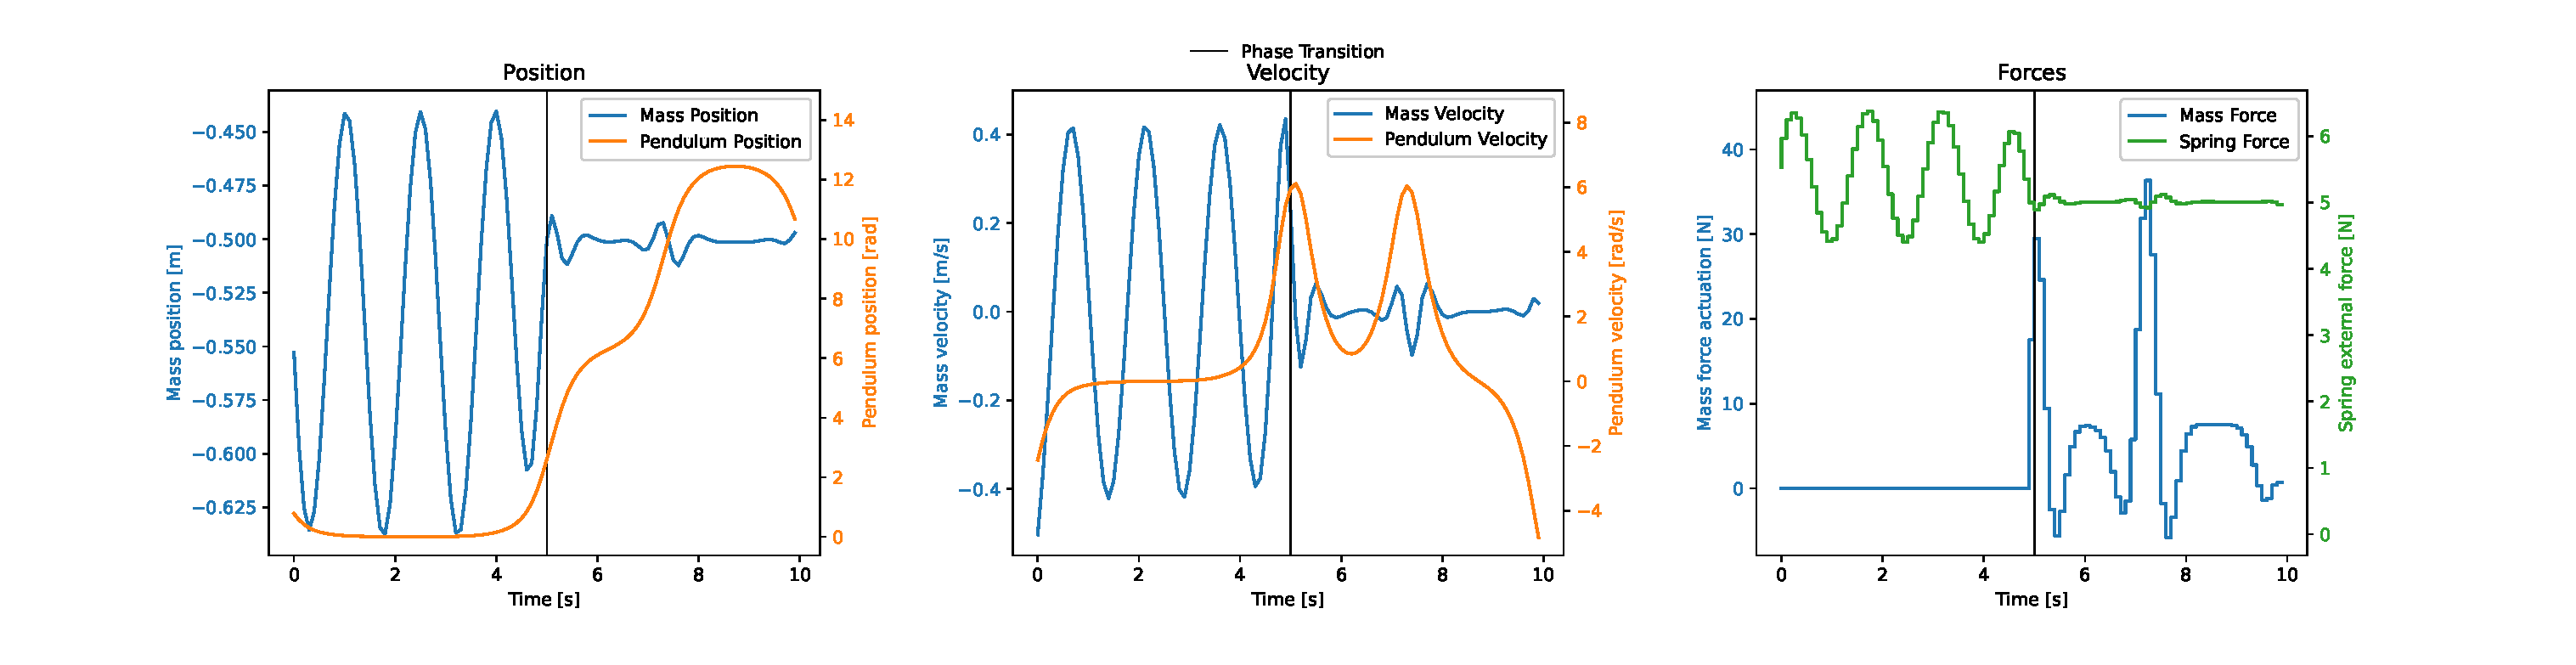
\includegraphics[width=\textwidth]{figures/Mass_Pendulum_Fext.eps}
\caption{Two-phases kinematics of the mass-pendulum-spring system. Gray dashed lines show the phase transition, blue lines are related to the mass (position velocity and external force acting on it), red lines are related to the pendulum (position and velocity) and the green line depicts the spring force.}
\label{fig:Mass_Pendulum_Fext_graphs}
\end{figure*}
















\subsection{Multiphase torque driven walking cycle}\label{ex:walking}
This walking example is presented to introduce \textit{bioptim}'s ability to deal with gait biomechanics as a multiphase problem with contact forces.
The goal was to estimate muscles activation by tracking markers trajectories, ground reaction forces and moments (Equations.~\ref{eq:ocp_markers}, ~\ref{eq:ocp_forces} and ~\ref{eq:ocp_moments}, respectively). 
The model was driven by muscle activation. 
To predict muscle activity, the objective function consisted in finding the least squared muscle activations $a_{i}$ (Equations.~\ref{eq:ocp_muscles}). 
Pure residual torques were also added to compensate potential underactuation from the model weaknesses and penalized as shown in equation ~\ref{eq:ocp_torques}.\\
The gait cycle was defined from the first heel strike to the end of the swing phase using a simplified 3D one-leg model with 12 DoFs and 17 muscles (pelvis + right lower limb). 
Based on experimental force plateform data and markers position, the stance was divided into three phases (heel, flatfoot and forefoot contacts) of fixed duration (0.05, 0.355 and 0.16s), to follow the natural rolling movement of the foot from heel strike to toe off.
The swing phase lasted 0.38 s. 
The interaction between the ground and the foot was modelled using a 4-contact points model located at the heel and the forefoot (first, fifth metatarsi and hallux).

The complete cycle was discretized in 90 intervals and the objective functions are written as follow :\\

%\[ 
%\resizebox{0.9\columnwidth}{!}{$ 
%\begin{aligned}
%\mathcal{J} = &\int_{t=0}^{T}\underbrace{\omega_1(\|m_p - m_m\|^{2})}_{\mathtt{TRACK\_MARKERS}}~ 
%+ ~ \underbrace{\omega_2(\|f_p - f_c\|^{2})}_{\mathtt{TRACK\_FORCES}}\\
%&+ ~ \underbrace{\omega_3(\|tau^f_p - tau^f_m\|^{2})}_{\mathtt{TRACK\_MOMENTS}}~
%\mathcal{J} = &\int_{t=0}^{T}\underbrace{\omega_1(\|m_p - m^*_m\|^{2})}_{\mathtt{TRACK\_MARKERS}}~ 
%+ ~ \underbrace{\omega_2(\|f_p - f^*_c\|^{2})}_{\mathtt{TRACK\_FORCES}}\\
%&+ ~ \underbrace{\omega_3(\|tau^f_p - tau^{f*}_m\|^{2})}_{\mathtt{TRACK\_MOMENTS}}~
%+ ~ \underbrace{\omega_4\|a\|^2}_{\mathtt{MIN\_ACTIVATION}}~dt, 
%\end{aligned}  
%$}  
%$}
%\addtag  
%\label{eq:ocp_walk}  
%\]

\begin{eqnarray}
\label{eq:ocp_markers}
\mathcal{J} = \sum_{i=1}^{N_i}\Bigg(\underbrace{\omega_1(\|m_p - m_m\|^{2})}_{\mathtt{TRACK\_MARKERS}}
\end{eqnarray}
\begin{eqnarray}
\label{eq:ocp_forces}
+ \underbrace{\omega_2(\|\sum_{c=1}^{N_c}F_p - F_m\|^{2})}_{\mathtt{TRACK\_FORCES}}
\end{eqnarray}
\begin{eqnarray}
\label{eq:ocp_moments}
+ \underbrace{\omega_3(\|\sum_{c=1}^{N_c}M_p - M_m\|^{2})}_{\mathtt{TRACK\_MOMENTS}}
\end{eqnarray}
\begin{eqnarray}
\label{eq:ocp_muscles}
+ \underbrace{\omega_4\int_0^T \sum_{i=1}^{N_i}~a_{i}^2~dt}_{\mathtt{MINIMIZE\_ ACTIVATION}})  
\end{eqnarray}
\begin{eqnarray}
\label{eq:ocp_torques}
+ \underbrace{\omega_5\int_0^T \sum_{i=1}^{2}~\tau_{i}^2~dt}_{\mathtt{MINIMIZE\_ TORQUE}}\bigg)
 \end{eqnarray}

where $\omega_{i}$ are the weighting factors ($\omega_1$=1e5, $\omega_2$=0.1, $\omega_3$=0.1, $\omega_4$=10, $\omega_5$=1), $T$ is the the duration, $N_i$ and $N_c$ are the number of time frames and contact points of the current phase. The indices $_p$ and $_m$ stand for predicted and measured data.\\

Non-slipping ($\mathtt{NON\_SLIPPING}$) and unilateral contact force ($\mathtt{CONTACT\_FORCE}$) constraints prevented the foot from slipping and pulling from the ground. 
In between phases, the use of the $\mathtt{IMPACT}$ state transition allowed to represent the gain or loss of contact(s) in the dynamics (e.g., swing phase to heel strike [thesis Felis - articles?]) \\

Fig.~\ref{fig:snapshots_multiphase_walking_cycle} shows the leg movements during the walking cycle. The mean tracking error on markers trajectories was 0.027 m (mean error on pelvic and foot markers was 0.0075 m and 0.0147 m, respectively). 
Concerning ground reaction forces tracking, the mean error was 4.85 N with an average $R^2$ at 0.9. 
Gluteal muscles were only activated during the stance phase and especially during the early flatfoot phase for the gluteus maximus with a maximal activation of 0.2. 
For the thigh muscles, the semimembranous, semitendinous and biceps femoris were activated during the early stance phase and terminal swing (maximal activation of 0.3, 0.4 and 0.4, respectively). 
The knee extensors, vastus lateralis, medialis and intermedius followed the same pattern and were mainly activated during the flatfoot phase. 
However, maximal activation of the rectus femoris appeared at early forefoot phase and early swing. Leg muscles were highly activated (saturation of gastocnemius lateralis and medialis) at the end of the stance and the early swing phase. 

\begin{figure*}[t!]
\centering
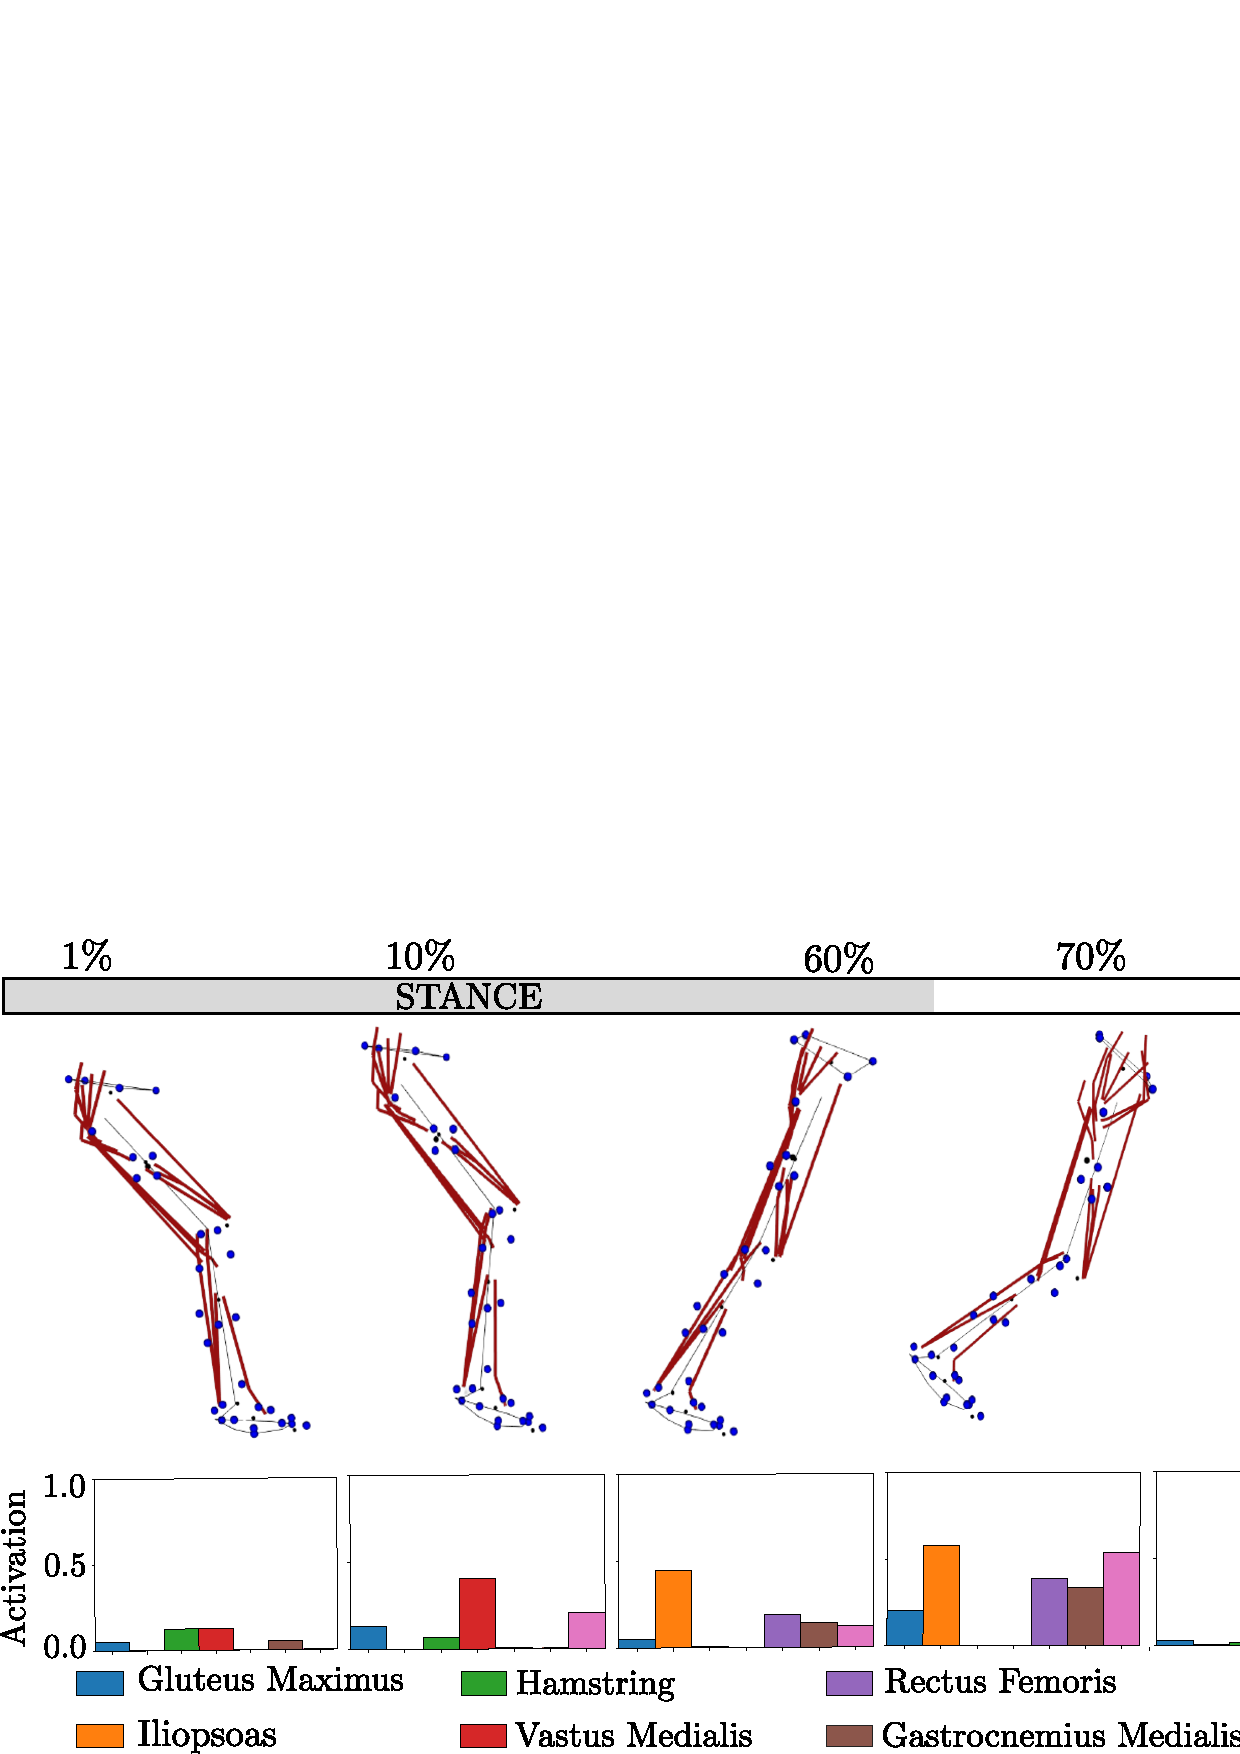
\includegraphics[width=\textwidth]{figures/multiphase_walking_cycle.png}\\
\caption{Snapshots of a walking gait cycle driven by muscles activation.}
\label{fig:snapshots_multiphase_walking_cycle}
\end{figure*}

%\begin{table}[h!]
%\caption{\small Objective terms of the Multiphase torque driven walking cycle }
%\label{tab:Multiphase_torque_driven_walking_cycle}
%\centering
%\begin{tabular}{c c c c}
%\toprule 
%& Type & Function & Weight \\ 
%\midrule
%$\#1$ & Lagrange & TRACK\_ STATE & $1e5$ \\ 
%\midrule
%$\#2$ & Lagrange & MINIMIZE\_ TORQUE\_ DERIVATIVE & $1e-2$ \\ 
%\midrule
%$\#3$ & Lagrange & TRACK\_ GRF & $1e-2$ \\ 
%\midrule
%$\#4$ & Lagrange & TRACK\_ MOMENTS & $1e-1$ \\
%\bottomrule
%\end{tabular}
%\end{table}


\subsection{Moving Horizon Estimation of Shoulder Elevation}\label{ex:mhe}
The goal was to estimate real-time joint kinematic and muscle activation using a moving horizon estimation (MHE). The example is given for a shoulder elevation motion using a 4-DoFs arm actuated by 19 Hill-type muscles. To use MHE, the OCP was split into a succession of smaller one. Each objective function was written as:

\[
\resizebox{0.9\columnwidth}{!}{$
\begin{aligned} \noindent \mathcal{J} = \sum_{n}^{n + n_{mhe}}\underbrace{\omega_1´(\|q_{ref} - q_{est}\|^{2})}_{TRACK\_STATE} ~ + ~ \underbrace{\omega_2\int_t^{t+t_{mhe}} \sum_{i=1}^{8}~Q_{i}^2~dt}_{MINIMIZE\_ STATE} ~ + ~ \underbrace{\omega_3\int_t^{t+t_{mhe}} \sum_{i=1}^{19}~U_{i}^2~dt}_{MINIMIZE\_ ACTIVATION} 
\end{aligned}
$} \addtag \label{eq:ocp_exMHE} 
\]

\noindent where $\omega_1$ =1e4 , $\omega_2$ = 10, $\omega_3$ = 100, $n_{mhe}$ is the number of OCP shooting node and $t_{mhe}$ is OCP duration. $q_{ref}$, $q_{est}$, $Q_i$ and $U_i$ are respectively reference and estimate joints angles, states and muscles activations. \\  
The first term of the objective function (Eq.~\ref{eq:ocp_exMHE}) corresponds to tracking experimental joint angles. Second and third were added for states and muscle controls regularization. Thanks to the high similarity between successive problems, a warm-start strategy using previous solutions was implemented.  
 
 
The shoulder elevation movement was generated with co-activation on two antagonists' muscles groups (triceps, biceps). It lasted for 8s and was discretized using 800 shooting nodes. A windows size of 7 nodes which allows the estimator to run around 50Hz, four times faster than standard biofeedback (13Hz), was chosen. Whereas reference data were generated at 100Hz, only one in two frames was sent to the estimator to correspond with experimental conditions.
 
The estimator was able to forecast the movement kinematic (Fig.~\ref{fig:angulare_angle_MHE}) with a consistent dynamic (Fig.~\ref{fig:muscles_excitations_MHE}). Due to cocontraction, the estimated muscles activations are lower than reference motion activations but with similar pattern. 
\begin{figure*}[t!] 
\centering 
\includegraphics[width=\textwidth]{figures/joint_angles_MHE.pdf}\\ 
\caption{Time series of estimated joint angles (blue) and noisy reference joint angles (orange).} 
\label{fig:joint_angles_MHE} 
\end{figure*} 

\begin{figure*}[t!] 
\centering 
\includegraphics[width=\textwidth]{figures/Muscle_Forces_MHE.pdf}\\ 
\caption{Time series of estimated muscle forces (blue) and ground truth muscle forces (orange). 
Only the muscles with significative action (peaks force $>$ 15~N) are represented.
Muscle abbreviations stand for (from left to right and top to bottom): Triceps Long head, Lateral and Medial, Brachial, Brachioradialis, Deltoid Anterior and Middle, Infraspinatus, Subscapularis, Biceps Brachial Long and Short head.} 
\label{fig:muscle_forces_MHE} 
\end{figure*} 


\subsection{Multiphase vertical jumper}\label{ex:jump}
This example is presented to introduce \textit{bioptim}'s ability to \hl{XXX}.
The goal was to find a minimal-time push-off phase for a \hl{XXX-DoF torque-driven} model while maximizing its jump height ($h$).
The push-off (impulsion before take-off) was divided into two phases with the following properties: \textit{1)} two contact points (heel and toe), duration $\in [0.2, 1.0]s$ and \textit{2)} one contact (toe), duration $\in [0.05, 1.0]s$.
The joint actuators bounds were modeled using a custom nonlinear constraint to account for torque/angle/angular-velocity relationships using the \verb?gauss3p? function of \textit{biorbd} \comment{based on predetermined factors}{je ne comprends pas} (\ref{fig:graph_force_vitesse_longueur}).
For each phase, the objective function was formulated as follow:

\[
\mathcal{J} = XXX.
\addtag
\label{eq:cost_jumper}
\]

The first term of Eq.~\ref{eq:cost_jumper} corresponds to maximizing the jump height.
The second term of the objective function serves for finding a minimal-time solution.

Using \textit{ipopt}, the problem was first approximately solved using the BFGS hessian approximation for 200 iterations maximum.
Then, \comment{if this maximum number of iterations was reached}{ne parler que de la solution présentée. Est-ce que le max_iter a effectivement été atteint ?}, the solution was re-optimized, using a warm-start, with exact-hessian computations for up to 1000 iterations .

The optimized ump height was 1,35m in \hl{XXX}s.
\comment{The used strategy is XXX with a proximo-distal shift of the joints (hip, knee then ankle) highlighted by the activation of the hip, then the knee and finally the ankle.}{à terminer}

\begin{figure}[h!]
\includegraphics[width=\columnwidth]{figures/graph_force_vitesse_longueur.png}\\
\caption{Surface representing the nonlinear constraint which account for torque/angle/angular-velocity relationships in the model of the jumper.}
\label{fig:graph_force_vitesse_longueur}
\end{figure}

%
\begin{table*}[h!]
\caption{\small Overview of computational results for the different OCPs cases and links to detailed implementations. The single shooting state trajectory is obtained by forwardly integrating the initial state with the optimized control inputs during 1~second. The single shooting error is computed as the mean RMSE between the optimized state vector and the single shooting one at 1~second.}
\label{tab:Perfs_and_detailed_implementations_of_each_example}
\centering
\begin{tabular}{c l rl rl rl}
\cmidrule[\heavyrulewidth](lr){2-8}
& & \multicolumn{2}{l}{\ref{ex:poiting} Activation-driven pointing} & \multicolumn{2}{l}{Ex\# 2} & \multicolumn{2}{l}{Ex\# 3} \\
\cmidrule[\heavyrulewidth](lr){3-4}
\cmidrule[\heavyrulewidth](lr){5-6}
\cmidrule[\heavyrulewidth](lr){7-8}

\mymultirow{4}{Setup} & \# states $\xt$            & \multicolumn{2}{c}{4}  & --    & --     & --    & --\\
                      & \# control $\ut$           & \multicolumn{2}{c}{6}  & --    & --     & --    & --\\
                      & \# shooting nodes          & \multicolumn{2}{c}{50} & --    & --     & --    & --\\
                      & OCP duration (s)           & \multicolumn{2}{c}{2}  & --    & --     & --    & --\\
                      &                            & \ipopt  & \acados        & \ipopt  & \acados  & \ipopt  & \acados \\
\mymultirow{3}{Solve} & \# NLP iterations          & 47     & 19            & --    & --     & --    & --\\
                      & Optimized cost             & 20.8 & 23.2        & --    & --     & --    & --\\
                      & Time to convergence (s)    & 22.3    & 0.45          & --    & --     & --    & --\\
                      & Single shooting error    & $<10^{-7}$    & $<10^{-13}$          & --    & --     & --    & --\\
%Example & Link & IPOPT & ACADOS \\ 

%\midrule
%Muscle activation driven pointing task & \href{https://github.com/pyomeca/BiorbdOptim/blob/master/examples/muscle_driven_ocp/static_arm.py}{$\star$} & $10.10$ & $0.2018$  \\ 
%\midrule
%$\bullet$ & $\bullet$ & $\bullet$ & $\bullet$ \\ 
\cmidrule[\heavyrulewidth](lr){2-8}
\end{tabular}
\end{table*}
%









\section{Discussion}\label{sec:discussion}
The purpose of \textit{bioptim} is to solve a variety of biomechanical OCPs with minimal user effort and high performances in terms of computational time. 
The main features illustrated by the six provided examples are (Tab.~X): 
\textit{i)} the possibility to use torque-, activation- or excitation-driven models (and their combinations);
\textit{ii)} a variety of ready-to-use cost functions, constraints and dynamics (with and without contacts)...;
\textit{iii)} ... easily customizable in Python when required by the user;
\textit{iv)} the possibility to solve advanced OCPs (possibly multi-phased) in a few seconds or minutes, that were previously known to take hours; 
\textit{v)} the interface with two different NLP solvers.
In the following, several aspects of \textit{bioptim} are discussed.

\subsection{Direct multiple shooting-based}

While the debate remains about the performances of direct collocations versus DMS \cite{diehl2006fast}\hl{[donner d'autres favorables a DC]}, the development of \textit{bioptim} was oriented toward DMS, because: \textit{i)} it allows to select effortlessly an arbitrary accuracy for the integration (e.g., number of RK steps); \textit{ii)} it allows to use DMS-based fast NLP solvers such as \textit{acados}.
Concerning the integration, either internally or via \textit{acados}, several schemes are implemented in \textit{bioptim} (RK4, RK8, IRK).
While IRK showed better convergence in our experience with hard problems in \textit{acados}, in most of the cases, RK4 showed to be a good speed/robustness trade-off. 
In contrast to what is claimed in several papers [\addref], DMS is not a limitation to the performances (cost value and time to convergence), since the performances of \textit{bioptim} often outperform state-of-the-art results.

\subsection{Automatic differentiation}

One of the reasons explaining the performances of \textit{bioptim} is the rewriting of the core software, \textit{RBDL} and \textit{biorbd} implementing the dynamics, into \textit{casadi} symbolics for automatically providing the exact Jacobians and Hessians of the resulting NLP.  
This feature is somewhat more computationally expensive than finite differences, but the gain in precision for the calculation of derivatives often leads to shorter convergence times (due to much less iterations) and to optimal solutions reached with lower tolerances.
This last aspect must be emphasized for complex motions (fast, highly dynamics ones), because talking about \textit{ipopt} for instance, an optimal solution obtained with a convergence criterion of $1e-2$ is very unlikely to be dynamically consistent (it would diverge when forward integrating the controls in a single-shooting manner), whereas a lower tolerance ($1e-6$. $1e-8$) only reachable with exact derivatives could lead to better forward dynamics results.

\subsection{Python based but fast!}

\textit{bioptim} was thought as an interface, and was therefore written in Python to allow the user to easily combine existing cost functions or constraints and self-implemented ones, to switch from one solver to another, etc. 
We believe this feature to be of importance given that the biomechanics community is known to be mainly made of software users rather than developers.
Therefore, providing a custom interface in Python rather than in, e.g., C++ [MOCO], was a driving objective of our work.
But since flexibility and ease-of-use should not compromise the performances, all the inside computations are expressed as C++ CasAdi graphs, interfaced with C++ NLP solvers.
These graphs can either be built in \texttt{casadi.MX()} or \texttt{casadi.SX()}.
\textit{acados} requires the latter, needing more RAM for building the problem but being faster to solve, whereas both options are available when using \textit{ipopt}. 
Inspired by the  real-time graphics from \textit{MUSCOD-II} \hl{[ref]}, \textit{bioptim} proposes a series of online-generated figures to analyze the iterations of the solvers with  minimal computational cost thanks to a \hl{XXX} protocole. 
Our implementation leverages the \textit{Python pickle} library for easily saving and loading OCPs for, e.g., post-processing analysis.

\subsection{Fast vs robust NLP solvers}

Fast solvers, such as \textit{acados}, offer the opportunity to use multi-start approaches on complex problems in order to circumvent the obstacle of local minima \cite{huchez2015local, bailly2020optimal} or to get meaningful initial solutions from simpler problems, for guiding the resolution of the harder problems.
On the other hands, robust solvers, such as \textit{ipopt}, are convenient when the user lacks information about the sought solutions and thus cannot guide the solver through a good initial guess.
For biomechanics applications, the complementary characteristics of the interfaced solvers is a really useful tool.

\subsection{Multiphase}

Biomechanics studies often face changing dynamics due to the loss or gain of contact or \hl{XXX}.
When tracking such a motion or trying to predict it, these dynamics changes translate into multi-phase OCP.
This is currently one of the drawbacks of \textit{moco}, which does not provide this feature.
\textit{bioptim}, however, is able to handle multi-phase OCPs, although they can currently only be solved with ipopt (see Ex. \hl{XXX} and \hl{XXX}).


\subsection{Cost vs constraints … relâcher le problème simplement}

\hl{???}

\subsection{Limitations}

Bioptim is already a mature solution for solving biomechanical OCP, however some limitations should be raised. 
First, it is based on  \textit{biorbd} which is actively maintained, fast and CasADi-compatible for automatic differentiation, but which is not as advanced as OpenSim or Anybody in terms of biomechanical features and audience. 
The variety of proposed examples highlighted simple to advanced models.
Even if defining a new model was made straightforward thanks to the \texttt{.bioMod} file format, \textit{biorbd} does not include a GUI for building models. 
Some Opensim models can be translated into \texttt{.bioMod} \hl{[LINK]} but our library does not yet support multiple wrapping objects, non-orthogonal DoFs between two bodies, compliant contact force models (e.g. [SmoothSphereHalfSpaceForce [52]]) or muscle-tendon equilibrium. 
As seen in \textit{Moco}, wrapping objects are rare due to computational cost and required optimization when a line of action is in contact with more than one object. 
Via points [\addref] and pre-processed moment arms (to be expressed as polynomial functions of crossed DoFs) are often preferred. 
\hl{In example X, the model differences (Opensim vs Biorbd), especially at the knee may explain the XXXX.} 

%Algorithms available in RBDL (core of biorbd for XXX) for ellipsoid foot model XXXXX (https://www.ncbi.nlm.nih.gov/pmc/articles/PMC6693511/).    

\subsection{Future directions}
Realtime estimation using MHE

MOOCP .. using front pareto

Prediction of adaptations due to muscular fatigue using NMPC

Muscle-tendon equilibrium and model builder are already planned and the former will either required an additional optimisation procedure to achieve the equilibrium as in CEINMS [\addref] or adding the length of muscle part with explicit constraints of XXXX in the OCP like in [\addref]. 

In line with the current studies of our research group, the future developments will first include \comment{nonlinear}{uniformiser l'écriture de ce mot} model predictive control and MHE (see example X) to predict optimal performances in repetitive tasks that generate muscular fatigue and real time estimation of joint torques and muscle forces, respectively. 
As shown in our previous studies [\addref] the analysis of a series near-optimal solutions is relevant in sport (but also in rehabilitation and ergonomics) and further efforts about multiobjective OCP of human performances are anticipated. 


\section*{Acknowledgment}
This study and the biorbd library development was partly funded by a scholarship of the  Vanier program (BM), the Canada First Research Excellence Fund via the TransMedTech Institute (FB) and the NSERC Discovey Programme (MB). 
Bioptim acts as a catalyst in our group and several students contributed to this library. 
Thank you to Paul, Théophile, Ariane, André and Kilpéric. 

\bibliographystyle{IEEEtran}
\bibliography{biblio}

\newpage
\input{sections/appendix}\label{sec:appendix}

\end{document}
